%=============================================================================
% SecureVoice --- IEEE conference paper (IEEEtran, two-column)
%
% Compile:  tectonic securevoice.tex
%      or:  pdflatex securevoice.tex  (run twice for references)
%      or:  upload this folder to Overleaf and select pdfLaTeX
%
% Figures expected in ../figures/ (generated by tools/build_figures.py)
%=============================================================================
\documentclass[conference]{IEEEtran}
\IEEEoverridecommandlockouts

\usepackage{cite}
\usepackage{amsmath,amssymb}
\usepackage{graphicx}
\usepackage{booktabs}
\usepackage{textcomp}
\usepackage{xcolor}
\usepackage[utf8]{inputenc}
\usepackage[T1]{fontenc}

\graphicspath{{../figures/}{figures/}}

% Rupee symbol without needing fontspec
\newcommand{\rs}{Rs.\,}

\begin{document}

\title{SecureVoice: Closing the Studio-to-Real-World Domain Gap\\
in Anti-Spoofing for Voice-Authenticated Transactions}

\author{
\IEEEauthorblockN{Atharva Kadge, Damodar Kamath, Shlok Kanvinde}
\IEEEauthorblockA{\textit{Department of Computer Engineering} \\
\textit{Sardar Patel Institute of Technology}\\
Mumbai, India}
}

\maketitle

%=============================================================================
\begin{abstract}
Voice-authenticated transaction systems increasingly rely on speaker
verification to answer ``is this the enrolled user's voice?'' but rarely ask
the different question, ``is this a real human?'' We build a two-layer
authorization pipeline---ECAPA-TDNN speaker verification plus AASIST-L
anti-spoofing---into a voice-ordering system and measure, rather than assume,
its security. Across 800 trials over 20 enrolled speakers on ASVspoof2019 LA,
54.0\% of synthetic voice-conversion/TTS attacks clear the speaker-verification
gate, while the anti-spoofing layer independently flags 87.0\% of them with
zero false alarms on genuine or impostor speech, cutting approved attacks to
7.5\% at typical transaction tiers. We then reproduce the anti-spoofing model's
published benchmark (0.99\% EER, matching the originally reported figure) and
document a severe practical failure: on our own real phone recordings, the same
model with the same frozen threshold misclassifies 100\% (8/8) of genuine
speech as synthetic. We diagnose this as a studio-versus-real-world domain
gap---ASVspoof2019's bona fide class is anechoic-chamber audio with a
16$\times$ lower noise floor and 10$\times$ more high-frequency energy than a
phone recording in an ordinary room---rule out codec, resampling, and gain
artifacts as the cause, and show that direct domain adaptation on a small set
of real recordings reduces the real-world false-positive rate from 8/8 to 2/8
at a measured, bounded cost to benchmark EER (2.00\%\,$\rightarrow$\,8.12\%).
We additionally quantify how the same model degrades under VoIP-style channel
loss (0.99\%\,$\rightarrow$\,14.00\% EER) and under short streaming windows
(0.99\%\,$\rightarrow$\,36.43\% at 250\,ms), and report all findings---including
negative results---under a fixed, development-set-only threshold-selection
protocol.
\end{abstract}

\begin{IEEEkeywords}
voice authentication, anti-spoofing, ASVspoof, speaker verification, domain
adaptation, AASIST, ECAPA-TDNN, deepfake speech detection
\end{IEEEkeywords}

%=============================================================================
\section{Introduction}

Personal voice assistants and voice-authenticated transaction systems
increasingly gate real financial actions---placing orders, moving money,
unlocking doors---behind a voice check~\cite{cheng2022survey}. Smart-speaker
adoption has grown rapidly and voice is now marketed as a convenience layer
atop e-commerce and banking flows, which means a successful attack on the voice
channel is no longer merely a privacy nuisance but a direct financial-fraud
vector. The dominant technical approach to securing that channel is speaker
verification (SV): compare an incoming utterance against an enrolled voiceprint
and approve if the cosine similarity of speaker embeddings clears a threshold.
SV answers ``is this the right voice?'' It does not answer ``is this a real
human speaking, or an AI-generated clone?''---a distinct question that a
determined attacker can now target cheaply with modern text-to-speech (TTS) and
voice-conversion (VC) tools, several of which are freely available and require
only a few seconds of reference audio.

This gap is not hypothetical. A clone is explicitly optimized to sound like the
target speaker, so a successful clone should, by construction, score well on
SV---its similarity should rise, not fall, relative to an unrelated impostor.
Prior surveys of the personal-voice-assistant (PVA) threat
landscape~\cite{cheng2022survey} identify voice authentication spoofing as a
mature but still-unresolved research area, and note that commercial assistants
rarely combine spoof detection with access control in practice. Meanwhile the
anti-spoofing research community has produced increasingly accurate
countermeasures---sub-1\% Equal Error Rate (EER) is now routine on the standard
ASVspoof benchmark~\cite{jung2022aasist}---creating an appealing but, as we
show, premature assumption that bolting such a model onto an SV pipeline solves
the problem.

We built \textit{SecureVoice}, a voice-ordering system secured by (i)
ECAPA-TDNN speaker verification~\cite{desplanques2020ecapa} and (ii) an added
anti-spoofing layer using AASIST-L~\cite{jung2022aasist}, a compact
(85k-parameter) graph-attention network benchmarked on the ASVspoof2019 Logical
Access (LA) corpus~\cite{todisco2019asvspoof}. Rather than assume the resulting
system is secure because each component is individually well-benchmarked, we
measured it end to end---against synthetic attacks, against degraded audio,
against short streaming windows, and, critically, against our own real voices
recorded on an ordinary phone in an ordinary room. That last test, originally
intended only as a pre-demonstration sanity check, produced this paper's
central finding: a model reporting 0.99\% error on its own benchmark
misclassified every one of our real recordings as synthetic, with high
confidence, using the same frozen operating threshold used everywhere else in
this work.

This paper's contribution is therefore as much methodological as architectural:
we show the value of testing a voice-security pipeline against the conditions
it will actually be deployed into, rather than stopping once each component
clears its own published benchmark. Concretely, we contribute:

\begin{itemize}
\item a measured, controlled demonstration that SV alone is insufficient
      against synthetic speech, using an 800-trial genuine/spoof/impostor
      protocol with authorization outcomes computed under a real transaction
      tier policy;
\item reproduction of a state-of-the-art anti-spoofing benchmark to validate
      our pipeline before trusting any downstream claim built on it;
\item an independent reproduction and diagnosis of the studio-to-real-world
      domain gap on consumer-device audio, with control experiments ruling out
      codec, resampling, and gain artifacts as the cause;
\item a lightweight domain-adaptation mitigation, reported honestly alongside a
      first attempt that failed, with its benchmark-accuracy cost quantified;
      and
\item quantification of the same model's degradation under realistic VoIP
      channel loss and short streaming windows, relevant to continuous rather
      than one-shot voice authentication.
\end{itemize}

Section~\ref{sec:lit} situates this work against prior voice-spoofing and PVA
security literature; Section~\ref{sec:method} details the system and
experimental protocols; Section~\ref{sec:results} reports and discusses
results; Section~\ref{sec:concl} concludes.

%=============================================================================
\section{Literature Survey}\label{sec:lit}

Voice authentication and its spoofing vulnerabilities have a long research
history predating current PVA deployments~\cite{cheng2022survey,wu2015survey}.
Five attack families are established: replay, impersonation, speech synthesis,
voice conversion, and adversarial perturbation. Replay attacks play back a
prerecorded genuine sample; synthesis and voice-conversion attacks instead
generate new audio designed to match a target voiceprint, and are the family
this paper concerns itself with, since modern TTS/VC pipelines make them cheap
to mount at scale. The ASVspoof challenge
series~\cite{todisco2019asvspoof,nautsch2021asvspoof,yamagishi2021asvspoof}
standardized datasets, protocols, and the EER and t-DCF~\cite{kinnunen2018tdcf}
metrics, distinguishing Logical Access (LA: synthesis/conversion attacks fed
directly to the verifier) from Physical Access (PA: replay through a real
microphone/loudspeaker channel). We scope this work to LA attacks; replay and
liveness detection is a related but distinct problem with its own countermeasure
literature~\cite{blue2018hello,zhang2016voicelive}.

\subsection{Benchmark Performance of Current Countermeasures}

AASIST~\cite{jung2022aasist} is a graph-attention network operating directly on
raw waveforms via a SincNet-style front end~\cite{ravanelli2018sincnet},
building on the earlier RawNet2~\cite{tak2021rawnet2} and
RawGAT-ST~\cite{tak2021rawgat} systems. Table~\ref{tab:sota} reproduces its
reported comparison on ASVspoof2019 LA. Sub-1\% EER is attainable, and notably
the 85k-parameter AASIST-L variant outperforms systems two orders of magnitude
larger, which is why we selected it for an on-device authorization setting.
ECAPA-TDNN~\cite{desplanques2020ecapa} is a widely adopted speaker-embedding
architecture producing fixed-dimension embeddings compared via cosine
similarity; we use it as SecureVoice's verification layer, matching common
practice of pairing a verification embedding model with a separately trained
countermeasure.

\begin{table}[t]
\caption{Published single-system results on ASVspoof2019 LA evaluation, as
reported in~\cite{jung2022aasist}. Reproduced for context; not our
measurements.}
\label{tab:sota}
\centering
\footnotesize
\begin{tabular}{@{}lrrr@{}}
\toprule
\textbf{System} & \textbf{\# Param} & \textbf{min t-DCF} & \textbf{EER (\%)}\\
\midrule
AASIST~\cite{jung2022aasist}            & 297k    & 0.0275 & 0.83\\
\textbf{AASIST-L}~\cite{jung2022aasist} & 85k     & 0.0309 & \textbf{0.99}\\
RawGAT-ST~\cite{tak2021rawgat}          & 437k    & 0.0333 & 1.19\\
SENet                                   & 1{,}100k & 0.0368 & 1.14\\
Res-TSSDNet                             & 350k    & 0.0481 & 1.64\\
Raw PC-DARTS~\cite{ge2021rawpcdarts}    & 24{,}480k & 0.0517 & 1.77\\
LCNN-LSTM-sum~\cite{wang2021comparative} & 276k   & 0.0524 & 1.92\\
\bottomrule
\end{tabular}
\end{table}

\subsection{The Generalization Problem}

A growing body of work questions whether these numbers survive outside the
challenge's own studio-recorded data. M\"uller et al.~\cite{muller2022generalize}
re-implement twelve architectures under a common protocol and evaluate them on
an ``In-the-Wild'' set of 37.9 hours of found audio from 58 celebrities and
politicians. They report EER degradations of 200--1000\%, with several models
collapsing to near chance (Table~\ref{tab:gap}). Critically for our work, they
attribute this to the composition of the benchmark itself, observing that
ASVspoof is built on the VCTK corpus~\cite{yamagishi2019vctk}, which
``exclusively features professional speakers and has been recorded in a studio
environment, using a semi-anechoic chamber.'' Related work by the same
group~\cite{muller2021silence} further suggests ASVspoof-trained models partly
key on non-speech cues such as leading and trailing silence rather than the
spoofing artefacts they are assumed to detect.

\begin{table}[t]
\caption{Benchmark-to-real-world EER degradation reported
by~\cite{muller2022generalize}. The final row shows their finding that
fixed-length 4\,s inputs underperform full-length inputs---directly relevant to
our streaming results (Section~\ref{sec:stream}).}
\label{tab:gap}
\centering
\footnotesize
\begin{tabular}{@{}lrrr@{}}
\toprule
\textbf{System} & \textbf{ASVspoof19} & \textbf{In-the-Wild} & \textbf{Degrad.}\\
\midrule
RawGAT-ST              & 1.23\%  & 37.15\% & 30$\times$\\
RawNet2                & 3.15\%  & 37.82\% & 12$\times$\\
12-model average       & 9.85\%  & 60.10\% & 6$\times$\\
Fixed 4\,s input (avg) & 18.89\% & 67.25\% & 3.6$\times$\\
\bottomrule
\end{tabular}
\end{table}

Our work is positioned deliberately with respect
to~\cite{muller2022generalize}: we do not claim to be first to observe that
anti-spoofing generalizes poorly. Rather, we contribute (i) an independent
reproduction of the phenomenon on a different class of real audio---%
self-collected, consent-based consumer-device recordings representing a
specific deployment context, rather than found celebrity media; (ii)
measurement of the downstream security consequence inside a working
authorization pipeline, which~\cite{muller2022generalize} does not address; and
(iii) a measured mitigation with its accuracy cost quantified. Prior work
establishes that the gap exists; we ask what it does to a deployed system and
what closing it costs.

Complementary defense families target different threat models. Channel-artifact
and second-factor defenses---detecting the sub-bass overexcitation
characteristic of loudspeaker playback~\cite{blue2018hello} or phoneme-timing
liveness cues~\cite{zhang2016voicelive}---address replay rather than synthesis,
and are complementary to, not substitutes for, the LA-focused defense studied
here. Zhang et al.~\cite{zhang2020mimicry} demonstrate a practical black-box
mimicry attack against a smart-home SV system, underscoring that SV alone is an
actively targeted attack surface. Feng et al.~\cite{feng2017continuous}
motivate continuous rather than one-shot voice authentication, a goal our
streaming experiments (Section~\ref{sec:stream}) show is nontrivial once a
fixed-input model is forced onto short windows.

%=============================================================================
\section{Proposed System and Methodology}\label{sec:method}

\subsection{Two-Layer Architecture}

SecureVoice authorizes a voice-issued transaction through two independent
checks that must both pass (Fig.~\ref{fig:arch}). \textbf{Layer 2} (speaker
verification) extracts a 192-dimension ECAPA-TDNN embedding and computes cosine
similarity against a centroid of enrollment embeddings (three short utterances
per user); similarity below 0.50 denies outright regardless of amount, and
above that floor a trust score ($100\times$similarity) is compared against a
minimum required for the requested transaction's risk tier. \textbf{Layer 2.5}
(anti-spoofing, our addition) scores the same raw audio independently with
AASIST-L; a synthetic-speech probability above a frozen threshold denies
regardless of Layer 2's outcome, so a perfect voice match cannot by itself
override a positive spoof detection. Both layers operate on 16\,kHz mono input
and add well under a second of combined latency on commodity hardware.

\begin{figure*}[t]
\centering
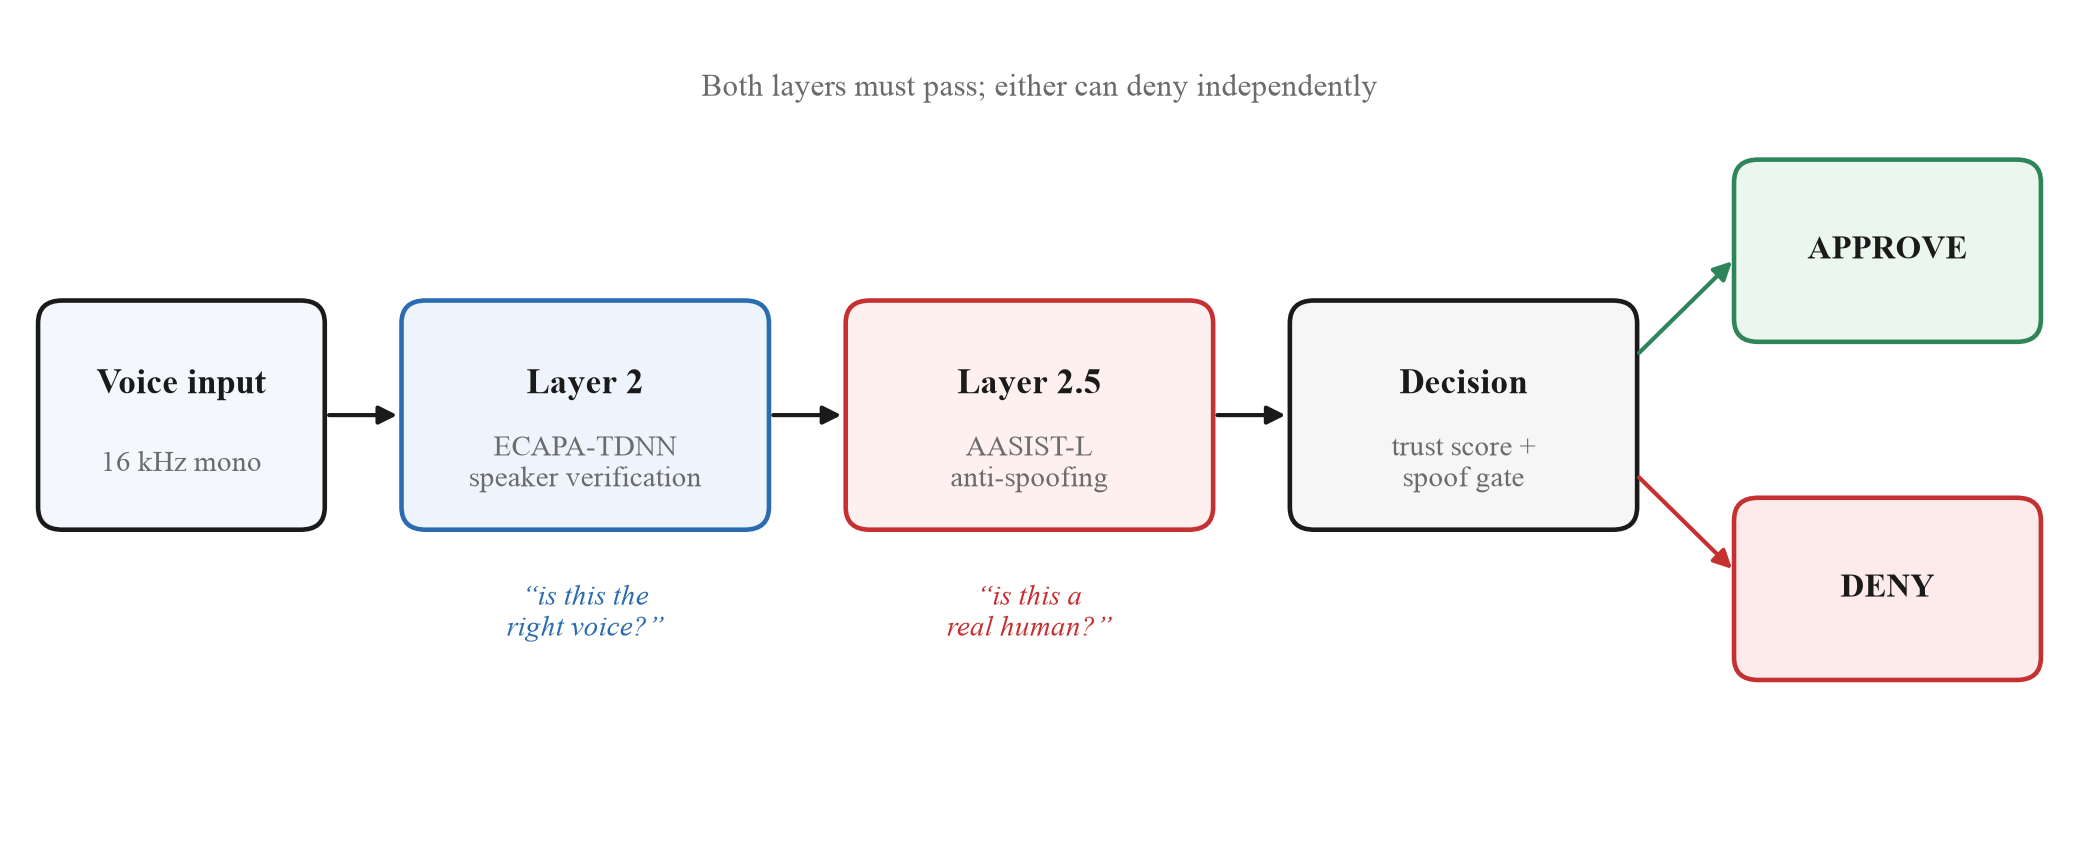
\includegraphics[width=0.86\textwidth]{fig1_architecture.png}
\caption{SecureVoice two-layer authorization pipeline. Layer~2 asks whether the
voice matches the enrolled user; Layer~2.5 (our addition) asks whether it is
human at all. Either layer can deny independently, so a perfect voice match
cannot override a positive spoof detection.}
\label{fig:arch}
\end{figure*}

\subsection{Threshold Discipline}

Every detector threshold is chosen on a held-out development split and frozen
before any evaluation-split or real-world number is produced, and is never
re-tuned per condition afterward, mirroring the discipline the ASVspoof
challenges impose on participants~\cite{nautsch2021asvspoof}. AASIST-L's
threshold is selected once by sweeping the ASVspoof2019 LA development split
for the EER operating point, then reused unchanged for every subsequent
experiment---including the real-world recordings, the degraded-channel
evaluation, and the streaming evaluation. This is what allows the failure in
Section~\ref{sec:gap} to be trusted as a genuine property of the model rather
than an artifact of a threshold quietly re-tuned after the fact.

\subsection{Vulnerability Measurement Protocol}

ASVspoof2019 LA labels every spoof utterance with the identity of the speaker
it targets, enabling a like-for-like enrolled-speaker comparison rather than a
pooled score. For 20 randomly drawn speakers, each enrolled from three held-out
bona fide utterances, we constructed three trial types: \textit{genuine} (ten
further held-out bona fide utterances of the same speaker), \textit{spoof}
(twenty TTS/VC attacks targeting that speaker), and \textit{impostor} (ten bona
fide utterances of a different speaker)---800 trials total. Each trial is
scored by both layers using their independently frozen thresholds; we report
the resulting similarity, spoof probability, and the authorization outcome both
with Layer~2.5 disabled and enabled, so the marginal value of anti-spoofing is
directly visible rather than inferred.

\subsection{Real-World Domain Gap: Discovery and Diagnosis}

After validating AASIST-L against its published benchmark
(Section~\ref{sec:repro}), we tested it on eight short assistant-style command
phrases recorded on an ordinary smartphone in a normal room---not through the
ASVspoof pipeline at all---purely as a sanity check before demonstrating the
live system. To diagnose the resulting failure rather than merely report it, we
compared long-term spectral energy distribution across five frequency bands and
a noise-floor estimate (10th-percentile short-time RMS over 25\,ms frames)
across ASVspoof bona fide audio, ASVspoof spoof audio, and our recordings. We
separately ran four control experiments---AAC compression at two bitrates,
16$\leftrightarrow$48\,kHz resampling, gain scaling, and mild additive noise
(30\,dB SNR) applied to clean ASVspoof bona fide audio---to test whether any
single easily-corrected signal-processing artifact could reproduce the failure.

\subsection{Domain Adaptation}

We attempted two mitigations, both starting from the original pretrained
checkpoint. \textbf{Fix~1} fine-tuned AASIST-L for two epochs on an ASVspoof2019
LA train subset (300 bona fide, 300 spoof) with synthetic room-reverb,
additive-noise, and microphone-frequency-response augmentation applied with
equal probability to both classes, so the augmentation distribution itself
could not become a shortcut label. \textbf{Fix~2} instead mixed six of our eight
real recordings directly into the same training mixture as additional bona fide
examples, oversampled fifteen times each with light gain and noise jitter to
avoid duplicate-sample memorization, while holding the remaining two clips out
entirely so any improvement on them could only come from genuine within-domain
generalization. Both were validated after every epoch on a fixed development
subset to confirm the model had not collapsed into a degenerate predictor, and
evaluated on a previously unseen 800-utterance evaluation subset for a
comparable benchmark-cost figure.

%=============================================================================
\section{Results and Discussion}\label{sec:results}

\subsection{Speaker Verification Alone Is Insufficient}

Table~\ref{tab:sv} summarizes the 800-trial protocol. ECAPA-TDNN is essentially
perfect against a different human speaker (0.00\% EER; no impostor clears the
0.50 gate) but far weaker against synthetic speech targeting the enrolled
speaker (18.62\% EER; 54.0\% of attacks clear the same gate). The same
embedding model, at the same threshold, behaves almost perfectly against one
threat model and only moderately better than chance against the other, because
it was never designed to distinguish ``a different real voice'' from ``a
synthesized copy of the target voice.'' In one representative case a clone
scored 0.799 similarity against the enrolled user's own 0.693---the fake
measuring as more authentic to the verifier than the genuine sample it was
cloned from.

\begin{table}[t]
\caption{Speaker-verification behavior by trial type ($n=800$, 20 speakers).}
\label{tab:sv}
\centering
\footnotesize
\begin{tabular}{@{}lrr@{}}
\toprule
\textbf{Trial type} & \textbf{Mean similarity} & \textbf{Clears 0.50 gate}\\
\midrule
Genuine ($n=200$)          & 0.726 & 99.5\%\\
Synthetic clone ($n=400$)  & 0.476 & \textbf{54.0\%}\\
Impostor ($n=200$)         & 0.124 & 0.0\%\\
\bottomrule
\end{tabular}
\end{table}

Adding the anti-spoofing layer flags 87.0\% of synthetic attacks with zero
false positives on genuine or impostor speech, cutting attacks approved at
low-value tiers from 54.0\% to 7.5\% (Table~\ref{tab:tiers},
Fig.~\ref{fig:attack}).

\begin{table}[t]
\caption{Synthetic attacks approved, by transaction tier.}
\label{tab:tiers}
\centering
\footnotesize
\begin{tabular}{@{}lrr@{}}
\toprule
\textbf{Tier} & \textbf{SV only} & \textbf{SV + anti-spoofing}\\
\midrule
$<$\rs500 / \rs500--2{,}000 & 54.0\% & \textbf{7.5\%}\\
\rs2{,}000--10{,}000        & 11.0\% & \textbf{1.8\%}\\
$>$\rs10{,}000              & 0.0\%  & 0.0\%\\
\bottomrule
\end{tabular}
\end{table}

\begin{figure}[t]
\centering
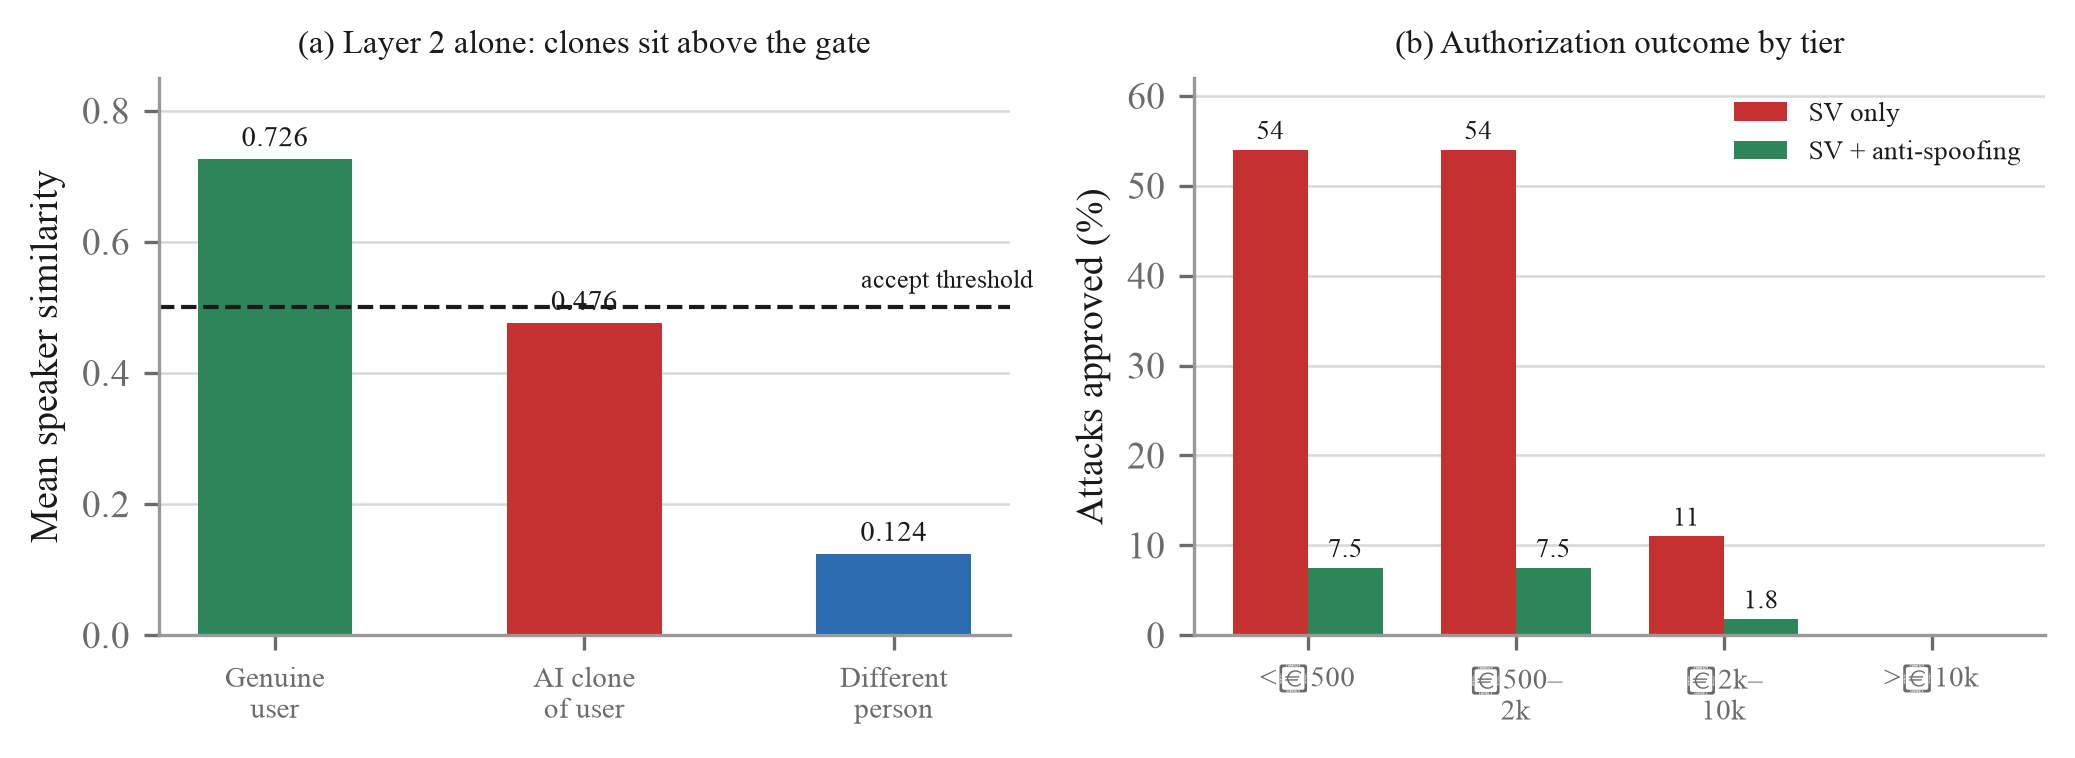
\includegraphics[width=\columnwidth]{fig4_attack.png}
\caption{(a) Mean speaker similarity by trial type: AI clones of the enrolled
user sit above the 0.50 accept threshold, whereas a different human never does.
(b) Share of synthetic attacks approved per transaction tier, with and without
the anti-spoofing layer.}
\label{fig:attack}
\end{figure}

\subsection{Benchmark Reproduction}\label{sec:repro}

Before trusting any downstream number we reproduced AASIST-L's published result
on the full ASVspoof2019 LA evaluation set (71{,}237 utterances): \textbf{0.99\%
EER}, matching the originally reported figure~\cite{jung2022aasist}
(Table~\ref{tab:sota}) against an 18.75\% EER classical LFCC-GMM baseline fit
on the same training split (LFCC-GMM development 9.38\%/evaluation 18.75\%;
AASIST-L development 0.51\%/evaluation 0.99\%). We include the weak classical
baseline not to contrast architectures for their own sake, but because its
larger degradation under the same stressors usefully calibrates how much of
AASIST-L's degradation is a property of the task versus the specific model.
This agreement is what makes the failure in Section~\ref{sec:gap} trustworthy
as a property of the model rather than a symptom of a broken evaluation
pipeline---a distinction that matters, since an unvalidated pipeline could
equally produce a spurious 100\% failure rate through a labeling bug.

\subsection{A Benchmark-Perfect Model Fails on Real Audio}\label{sec:gap}

All eight real phone recordings were misclassified as synthetic, every one
scoring above 0.98 probability against the frozen 0.9157 threshold
(Table~\ref{tab:fpr}). Spectral analysis (Table~\ref{tab:spectral},
Fig.~\ref{fig:gap}) shows why: real phone audio carries a 16$\times$ higher
noise floor and roughly 10$\times$ less 6--8\,kHz energy than ASVspoof's
anechoic-chamber bona fide class. The model had learned ``studio-clean,'' not
``human.'' Control experiments applying AAC compression, resampling, gain
change, or mild noise to lab audio did not reproduce the failure, ruling those
out as sole causes and implicating the recording environment and microphone
chain as a whole. This is consistent with~\cite{muller2022generalize}, obtained
independently on a different class of real audio.

\begin{table}[t]
\caption{Real-world false-positive rate on eight bona fide phone recordings,
before and after domain adaptation.}
\label{tab:fpr}
\centering
\footnotesize
\begin{tabular}{@{}lrr@{}}
\toprule
\textbf{Sample} & \textbf{Original model} & \textbf{Domain-adapted}\\
\midrule
8 real recordings & 8/8 flagged (100\%) & \textbf{2/8 flagged (25\%)}\\
\bottomrule
\end{tabular}
\end{table}

\begin{table}[t]
\caption{Spectral energy share and noise floor by source.}
\label{tab:spectral}
\centering
\footnotesize
\begin{tabular}{@{}lrrr@{}}
\toprule
\textbf{Band} & \textbf{Lab bona fide} & \textbf{Lab spoof} & \textbf{Real phone}\\
\midrule
0--300\,Hz  & 39.9\%  & 46.8\%  & \textbf{53.8\%}\\
6--8\,kHz   & 0.38\%  & 0.48\%  & \textbf{0.04\%}\\
Noise floor & 0.0043  & 0.0186  & \textbf{0.0702}\\
\bottomrule
\end{tabular}
\end{table}

\begin{figure}[t]
\centering
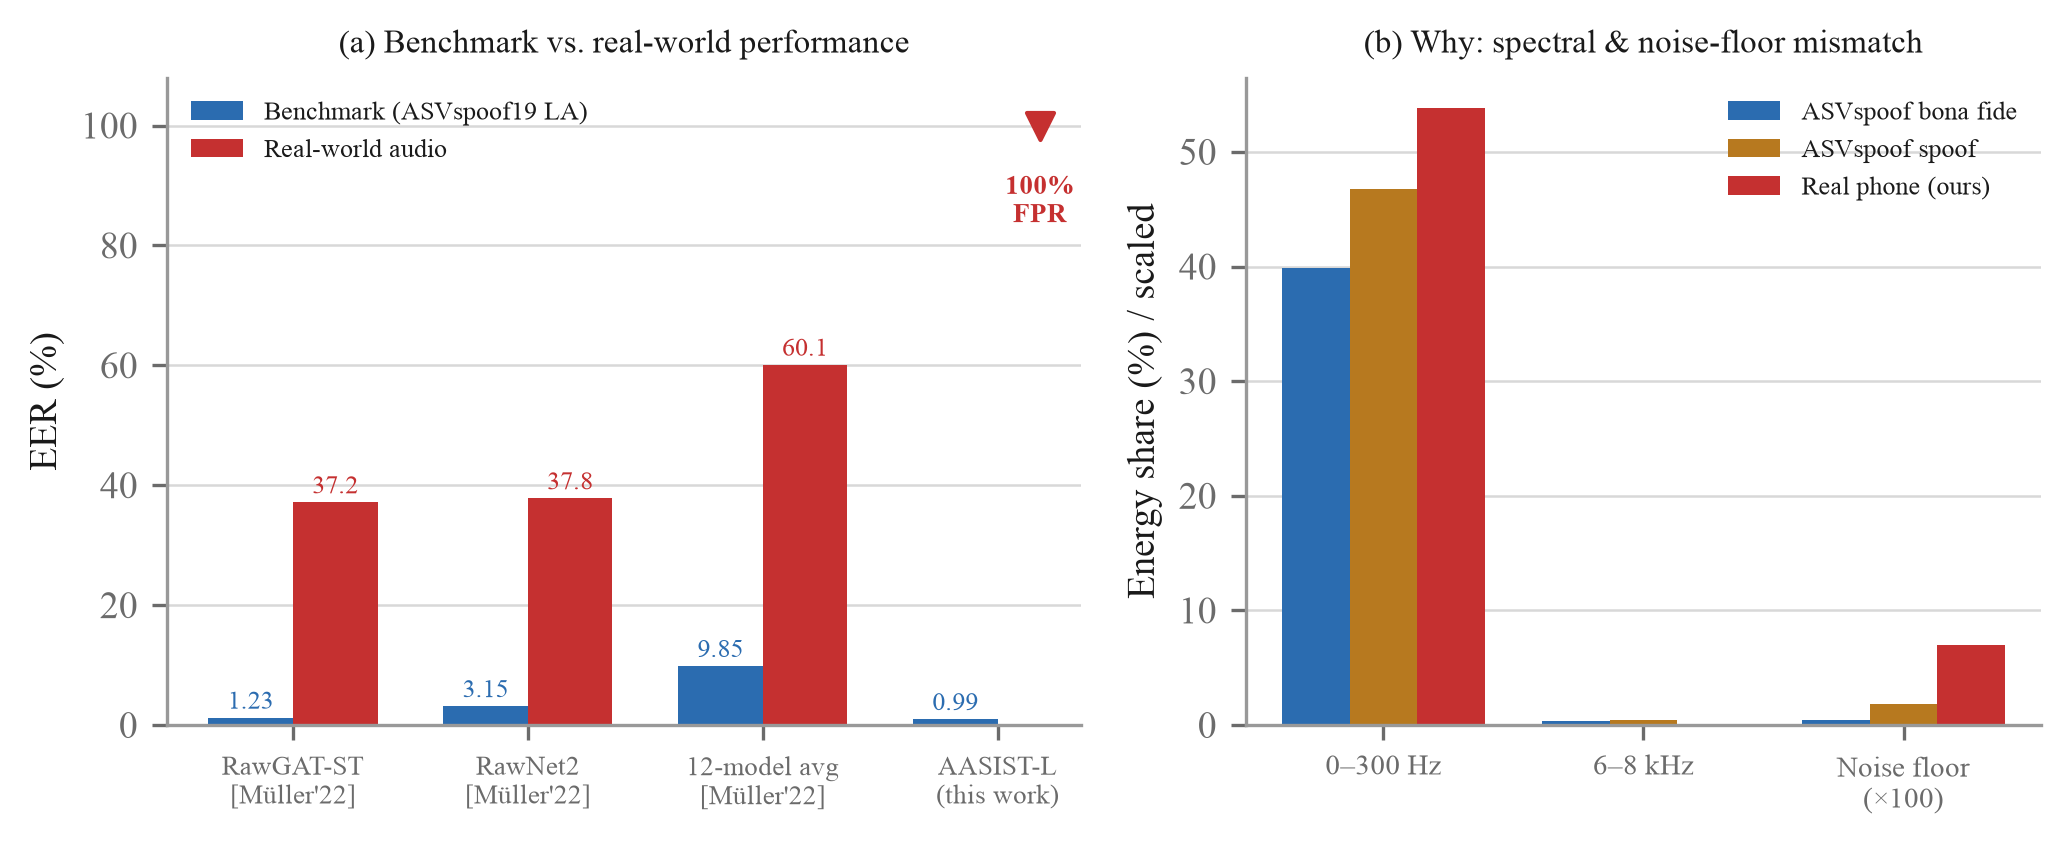
\includegraphics[width=\columnwidth]{fig2_domain_gap.png}
\caption{(a) Benchmark versus real-world performance. Literature values
from~\cite{muller2022generalize}; our AASIST-L benchmark EER is measured, and
its real-world figure is a 100\% false-positive rate on bona fide phone audio
(no EER is defined without in-domain attacks). (b) Spectral and noise-floor
mismatch underlying the failure.}
\label{fig:gap}
\end{figure}

\subsection{Mitigation: One Failure, One Success}

\textbf{Fix~1} improved EER on synthetically-degraded validation audio
(37.50\%\,$\rightarrow$\,18.33\% over two epochs) but did not transfer: real
recordings remained 8/8 misclassified with scores essentially unchanged
(0.93--0.99). We report this as a genuine negative result---approximated
augmentation is not a substitute for real-domain data at this scale.
\textbf{Fix~2} reduced real-world false positives to 2/8, and both held-out
clips, never seen during training, flipped from $>$0.94 to $<$0.05 probability
of being synthetic---a weak but genuine within-domain generalization signal.
The cost was a bounded rise in benchmark EER on a held-out 800-utterance
evaluation sample, from 2.00\% to 8.12\%. Importantly, the adapted model still
detects real attacks (the spoof clip of Section~\ref{sec:results} scores
0.99999). This is a small-scale proof of concept---one phone, one room, one
speaker---and not yet evidence of broad generalization.

\subsection{Robustness Under Channel Degradation}

Real voice traffic rarely reaches a back-end verifier as clean studio audio. We
simulated an Opus codec round-trip at three bitrates crossed with
Gilbert--Elliott burst packet loss at three rates on a class-balanced
3{,}000-utterance evaluation subsample, re-scoring both detectors with their
already-frozen thresholds (Table~\ref{tab:voip}, Fig.~\ref{fig:degrade}).
AASIST-L's advantage over the classical baseline collapses from 15.6$\times$ on
clean audio to 1.9$\times$ at the worst tested condition---the strong model
still wins, but its practical margin nearly disappears exactly under the
conditions a real VoIP transaction introduces.

\begin{table}[t]
\caption{EER under simulated VoIP channel degradation.}
\label{tab:voip}
\centering
\footnotesize
\begin{tabular}{@{}lrrr@{}}
\toprule
\textbf{Condition} & \textbf{LFCC-GMM} & \textbf{AASIST-L} & \textbf{Advantage}\\
\midrule
Clean                     & 18.30\% & 1.17\%  & 15.6$\times$\\
Opus 16\,kbps, 5\% loss   & 21.03\% & 5.23\%  & 4.0$\times$\\
Opus 8\,kbps, 15\% loss   & 26.83\% & 14.00\% & \textbf{1.9$\times$}\\
\bottomrule
\end{tabular}
\end{table}

\subsection{Robustness Under Short Streaming Windows}\label{sec:stream}

Continuous authentication implies scoring short chunks rather than complete
utterances, so we re-ran both detectors over non-overlapping 250, 500, and
1000\,ms windows (Table~\ref{tab:stream}). AASIST-L requires a fixed 4.04\,s
input, so shorter chunks are tile-repeated to fill it, discarding most temporal
structure---EER rises from 0.99\% at utterance level to 36.43\% at 250\,ms, an
accuracy collapse rather than graceful degradation. Adding packet loss on top
pushes AASIST-L to 38.70\% and the classical baseline past chance (45--55\%),
which we report as a genuine if unflattering finding. Per-chunk latency remained
real-time-capable throughout ($\approx$55\,ms, well under any tested window), so
the bottleneck is accuracy, not speed: naive chunking of a fixed-input model is
not a viable continuous-authentication strategy, and window-aware retraining,
not faster hardware, is the needed next step. This independently reproduces the
trend reported in~\cite{muller2022generalize}, where fixed 4\,s inputs
underperformed full-length inputs (Table~\ref{tab:gap}).

\begin{table}[t]
\caption{Chunk-level EER and latency versus window size (clean audio).}
\label{tab:stream}
\centering
\footnotesize
\begin{tabular}{@{}lrr@{}}
\toprule
\textbf{Window} & \textbf{AASIST-L EER} & \textbf{Latency}\\
\midrule
Full utterance & \textbf{0.99\%}  & ---\\
1000\,ms       & 23.62\% & 55\,ms\\
500\,ms        & 33.28\% & 55\,ms\\
250\,ms        & 36.43\% & 58\,ms\\
\bottomrule
\end{tabular}
\end{table}

\begin{figure}[t]
\centering
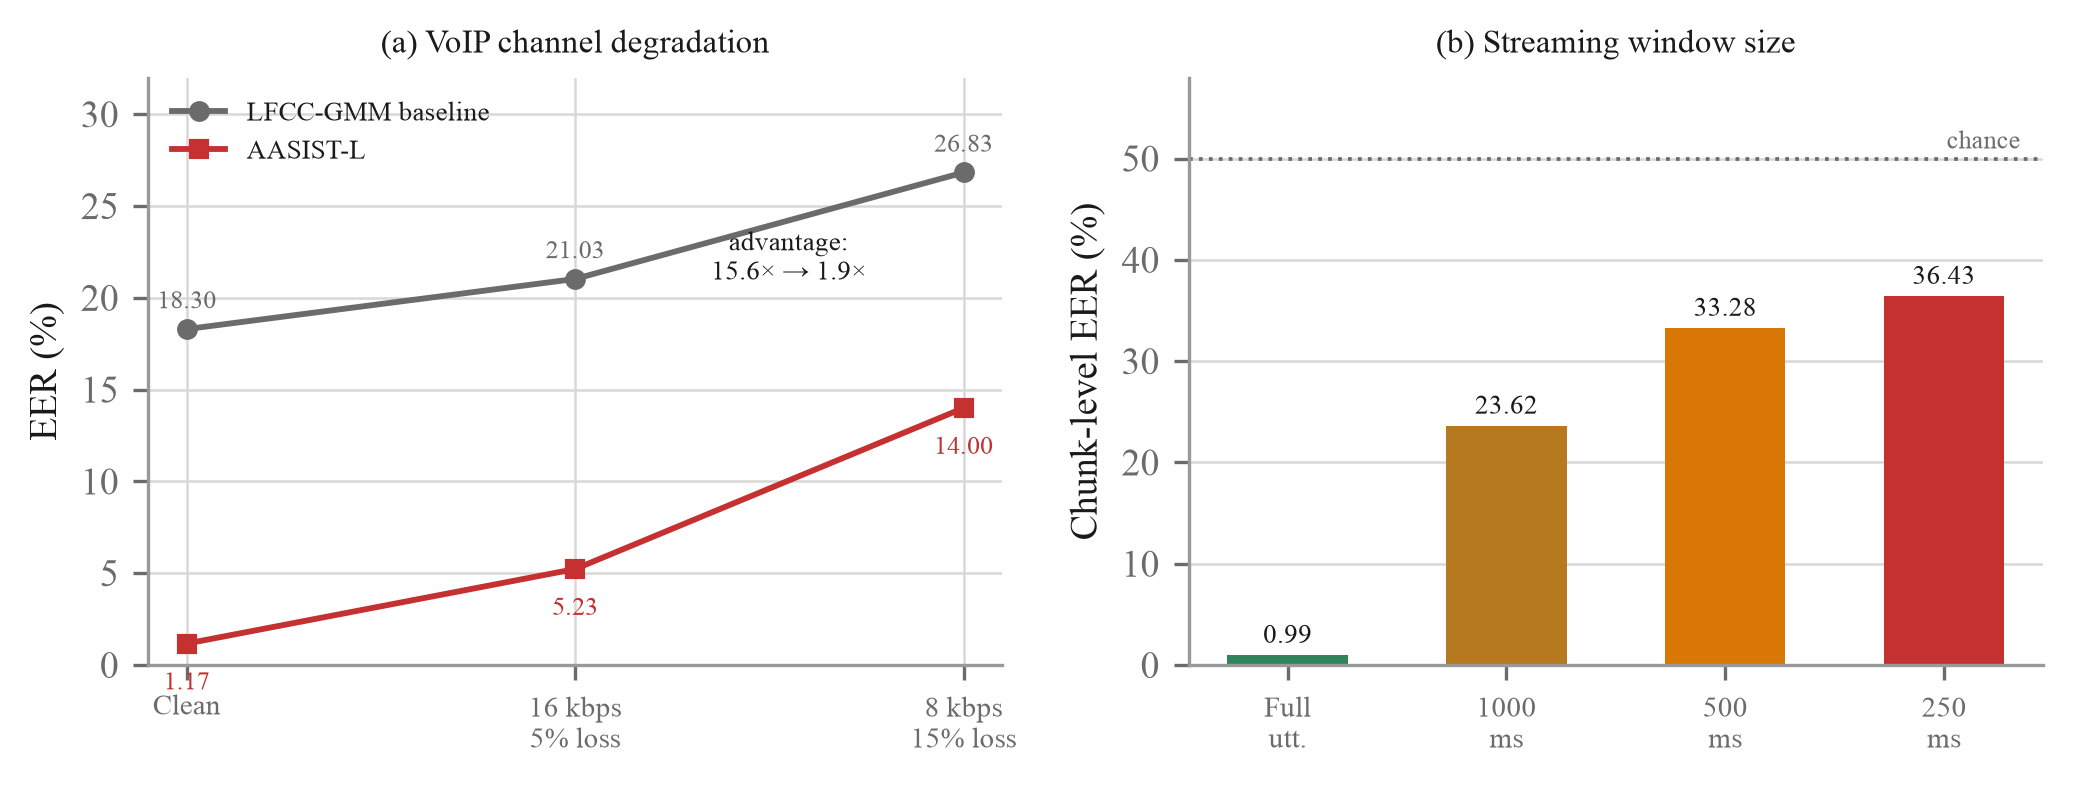
\includegraphics[width=\columnwidth]{fig3_degradation.png}
\caption{(a) EER under simulated VoIP channel degradation; AASIST-L's advantage
over the classical baseline narrows from 15.6$\times$ to 1.9$\times$.
(b) Chunk-level EER versus streaming window size on clean audio.}
\label{fig:degrade}
\end{figure}

\subsection{Limitations}

Our real-world evaluation uses eight recordings from a single speaker, device,
and room; it demonstrates the failure and a mitigation but does not establish
generalization across devices, rooms, or speakers. The attacks are ASVspoof2019
LA (2019-era TTS/VC), so the 54\% attack-success figure is likely a lower bound
against current cloning tools. VoIP degradation is simulated rather than
captured from live calls. Finally, the streaming results use naive
tile-repetition rather than a model retrained for short inputs.

%=============================================================================
\section{Conclusion and Future Work}\label{sec:concl}

Speaker verification alone approved over half of the synthetic-voice attacks we
tested; a benchmarked anti-spoofing layer closes most of that gap. More
consequentially, a model scoring 0.99\% EER on its own benchmark failed
completely on real-world audio---a gap we diagnosed spectrally and partially
closed via targeted domain adaptation at a measured accuracy cost. Future work:
scale domain adaptation across more speakers, devices, and rooms; evaluate
against modern post-2019 cloning tools; and pursue window-aware retraining for
genuinely streaming continuous authentication.

%=============================================================================
\begin{thebibliography}{20}
\footnotesize

\bibitem{cheng2022survey}
P.~Cheng and U.~Roedig, ``Personal voice assistant security and privacy---A
survey,'' \emph{Proc. IEEE}, vol.~110, no.~4, pp.~476--507, Apr. 2022.

\bibitem{todisco2019asvspoof}
M.~Todisco \emph{et al.}, ``ASVspoof 2019: Future horizons in spoofed and fake
audio detection,'' in \emph{Proc. Interspeech}, 2019, pp.~1008--1012.

\bibitem{nautsch2021asvspoof}
A.~Nautsch \emph{et al.}, ``ASVspoof 2019: Spoofing countermeasures for the
detection of synthesized, converted and replayed speech,'' \emph{IEEE Trans.
Biometrics, Behavior, and Identity Science}, vol.~3, no.~2, pp.~252--265, 2021.

\bibitem{yamagishi2021asvspoof}
J.~Yamagishi \emph{et al.}, ``ASVspoof 2021: Accelerating progress in spoofed
and deepfake speech detection,'' arXiv:2109.00537, 2021.

\bibitem{jung2022aasist}
J.-W. Jung, H.-S. Heo, H.~Tak, H.-J. Shim, J.~S. Chung, B.-J. Lee, H.-J. Yu,
and N.~Evans, ``AASIST: Audio anti-spoofing using integrated spectro-temporal
graph attention networks,'' in \emph{Proc. IEEE ICASSP}, 2022,
pp.~6367--6371.

\bibitem{desplanques2020ecapa}
B.~Desplanques, J.~Thienpondt, and K.~Demuynck, ``ECAPA-TDNN: Emphasized
channel attention, propagation and aggregation in TDNN based speaker
verification,'' in \emph{Proc. Interspeech}, 2020, pp.~3830--3834.

\bibitem{muller2022generalize}
N.~M. M\"uller, P.~Czempin, F.~Dieckmann, A.~Froghyar, and K.~B\"ottinger,
``Does audio deepfake detection generalize?,'' in \emph{Proc. Interspeech},
2022, pp.~2783--2787.

\bibitem{tak2021rawgat}
H.~Tak, J.-W. Jung, J.~Patino, M.~Kamble, M.~Todisco, and N.~Evans,
``End-to-end spectro-temporal graph attention networks for speaker verification
anti-spoofing and speech deepfake detection,'' arXiv:2107.12710, 2021.

\bibitem{ge2021rawpcdarts}
W.~Ge, J.~Patino, M.~Todisco, and N.~Evans, ``Raw differentiable architecture
search for speech deepfake and spoofing detection,'' arXiv:2107.12212, 2021.

\bibitem{wang2021comparative}
X.~Wang and J.~Yamagishi, ``A comparative study on recent neural spoofing
countermeasures for synthetic speech detection,'' in \emph{Proc. Interspeech},
2021, pp.~4259--4263.

\bibitem{muller2021silence}
N.~M. M\"uller, F.~Dieckmann, P.~Czempin, R.~Canals, J.~Williams, and
K.~B\"ottinger, ``Speech is silver, silence is golden: What do ASVspoof-trained
models really learn?,'' arXiv:2106.12914, 2021.

\bibitem{yamagishi2019vctk}
J.~Yamagishi, C.~Veaux, and K.~MacDonald, ``CSTR VCTK corpus: English
multi-speaker corpus for CSTR voice cloning toolkit (version 0.92),''
University of Edinburgh, 2019.

\bibitem{blue2018hello}
L.~Blue, L.~Vargas, and P.~Traynor, ``Hello, is it me you're looking for?
Differentiating between human and electronic speakers for voice interface
security,'' in \emph{Proc. ACM WiSec}, 2018, pp.~123--133.

\bibitem{zhang2016voicelive}
L.~Zhang, S.~Tan, J.~Yang, and Y.~Chen, ``VoiceLive: A phoneme localization
based liveness detection for voice authentication on smartphones,'' in
\emph{Proc. ACM CCS}, 2016, pp.~1080--1091.

\bibitem{zhang2020mimicry}
L.~Zhang, Y.~Meng, J.~Yu, C.~Xiang, B.~Falk, and H.~Zhu, ``Voiceprint mimicry
attack towards speaker verification system in smart home,'' in \emph{Proc. IEEE
INFOCOM}, 2020, pp.~377--386.

\bibitem{feng2017continuous}
H.~Feng, K.~Fawaz, and K.~G. Shin, ``Continuous authentication for voice
assistants,'' in \emph{Proc. ACM MobiCom}, 2017, pp.~343--355.

\bibitem{tak2021rawnet2}
H.~Tak, J.~Patino, M.~Todisco, A.~Nautsch, N.~Evans, and A.~Larcher,
``End-to-end anti-spoofing with RawNet2,'' in \emph{Proc. IEEE ICASSP}, 2021,
pp.~6369--6373.

\bibitem{ravanelli2018sincnet}
M.~Ravanelli and Y.~Bengio, ``Speaker recognition from raw waveform with
SincNet,'' in \emph{Proc. IEEE SLT}, 2018, pp.~1021--1028.

\bibitem{kinnunen2018tdcf}
T.~Kinnunen \emph{et al.}, ``t-DCF: A detection cost function for the tandem
assessment of spoofing countermeasures and automatic speaker verification,'' in
\emph{Proc. Odyssey}, 2018, pp.~312--319.

\bibitem{wu2015survey}
Z.~Wu, N.~Evans, T.~Kinnunen, J.~Yamagishi, F.~Alegre, and H.~Li, ``Spoofing
and countermeasures for speaker verification: A survey,'' \emph{Speech
Communication}, vol.~66, pp.~130--153, 2015.

\end{thebibliography}

\end{document}
